\chapter{Tabelas/Gráficos}

    \setcounter{section}{0}

    \begin{figure}[H]
      \centering
      \begin{tikzpicture}
          \begin{axis}
            [xbar interval,
            xmax=92,xmin=16,
              minor x tick num = 5,
              yticklabels=\empty,
              xlabel={idade},
              ]
            \addplot+[ 
            boxplot prepared={
              median=55,
              upper quartile=55,
              lower quartile=47,
              upper whisker=26,
              lower whisker=82
            },
            ] coordinates {};
          \end{axis}
      \end{tikzpicture}
      \caption{Box Plot}
    \end{figure}

    O boxplot apresentou resultados interessantes, todas as variáveis presentes na 
    amostra de idades não ultrapassam dos outliers estabelecidos. Além disso se 
    apresenta os valores 47, 55 e 61 para os quartis respectivamente.        

    \begin{figure}[H]
        \centering
        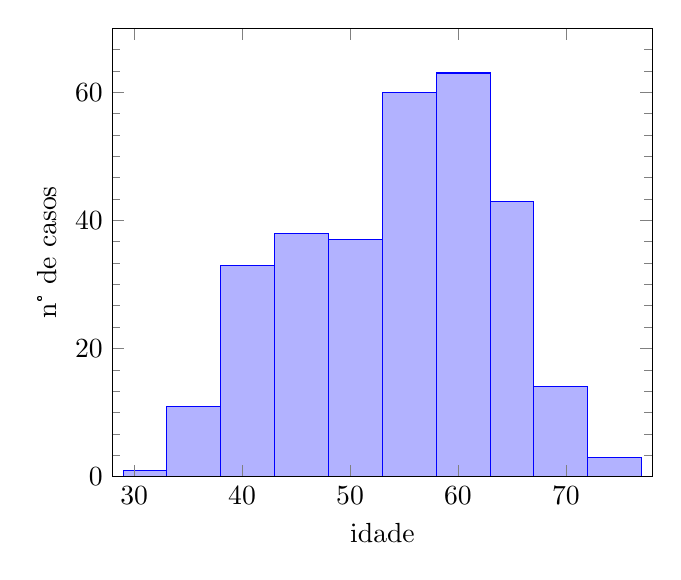
\begin{tikzpicture}
            \begin{axis}[
                xlabel={idade},
                ylabel={n° de casos},
                ymin=0, ymax=70,
                xmin=28, xmax=78,
                minor y tick num = 5,
                area style,
                ]
                \addplot+[ybar interval, mark=no] plot coordinates { (29, 1) (33, 11) (38, 33) (43, 38) (48, 37) (53, 60) (58, 63) (63, 43)  (67, 14)  (72, 3)  (77, 3)};
            \end{axis}
        \end{tikzpicture}
        \caption{Histograma}    
    \end{figure}

    Com o histograma, podemos observar uma ocorrência maior de casos em pessoas com 
    faixa etária entre 50 à 65 anos. A presença de casos para pessoas abaixo de 30 
    anos e acima dos 80 anos é quase nula.
